\section{Materiais e métodos}

\subsection{Intel RAPL}
\begin{frame}{Intel RAPL}
    \begin{itemize}
        \item Otimizar o gerenciamento energético dos processadores Intel
        \item Monitoramento de alguns parametros como temperatura, potência e consumo energético
        \item Foi implementado a nível de hardware a partir da 6ª geração dos processadores Intel
        \item Segundo Khan at al 2018 \cite{khan2018IntelRapl}, a precisão do RAPL é bastante promisora e os valores reportados são precisos suficientemente para prever e modelar sistemas.
    \end{itemize}
\end{frame}

\begin{frame}{RAPL Power Domain}
    \begin{figure}
        \centering
        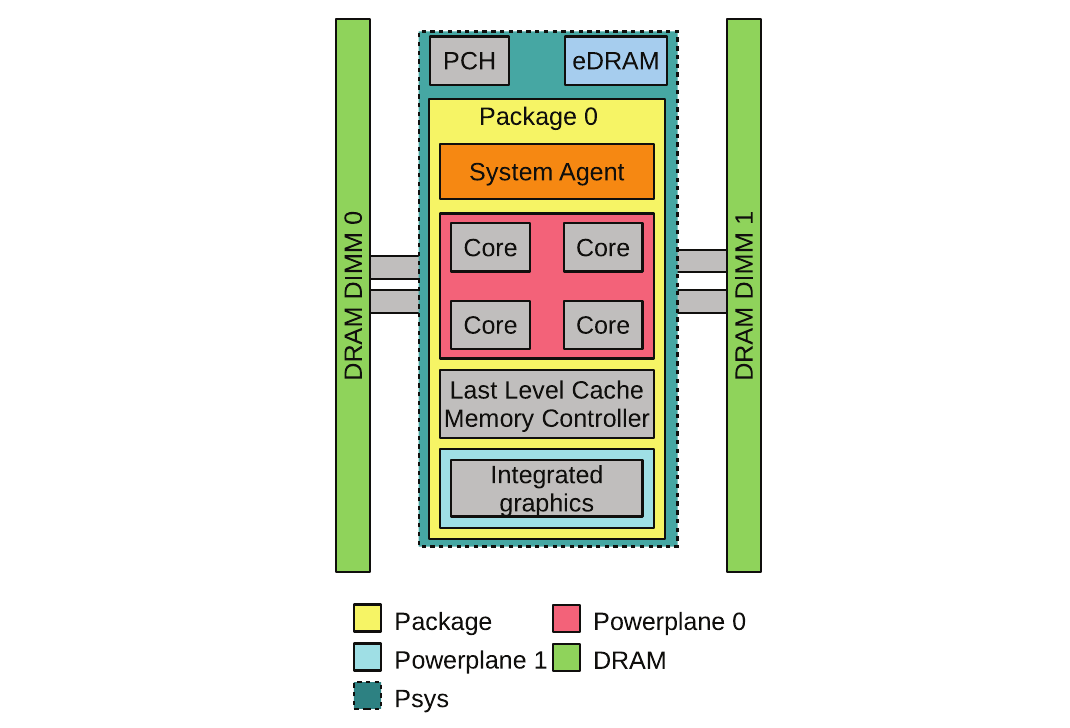
\includegraphics[width=0.61\linewidth]{images/powerDomainsRAPL.png}
        \caption{Intel RAPL Power Domains. Fonte: Khan at al 2018 \cite{khan2018IntelRapl}}
        \label{fig:powerDomains}
    \end{figure}
\end{frame}

\begin{frame}{Gerações E suporte ao RAPL dos Processadores Intel}
        \begin{figure}
            \centering
            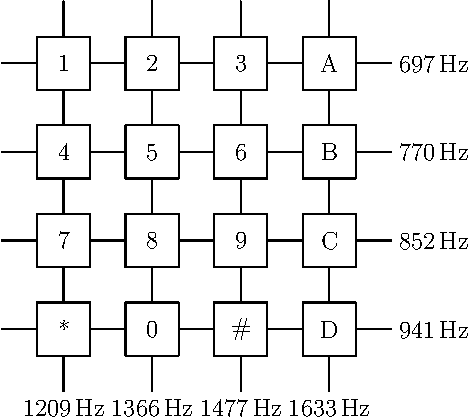
\includegraphics[width=0.35\linewidth]{images/dtmf.pdf}
            \caption{Exemplo de um PDF incluído em um frame}
            \label{fig:example}
        \end{figure}
\end{frame}

\subsection{GNU Time}
\begin{frame}{GNU Time}
    \begin{itemize}
        \item A
        \item B
        \item C 
        \item D 
    \end{itemize}
\end{frame}

\subsection{Shell}
\begin{frame}{Shell}
    \begin{itemize}
        \item A
        \item B
        \item C 
        \item Shell scripts
        \item Bash
    \end{itemize}
\end{frame}

\subsection{The Computer Language Benchmark Game}
\begin{frame}{The Computer Language Benchmark Game}
    \begin{itemize}
        \item A
        \item B
        \item C 
        \item D 
    \end{itemize}
\end{frame}

\subsection{Linguagens de Programação}
\begin{frame}{Linguagens de Programação}
    \begin{table}[h]
        \centering
        \fontsize{6}{7}\selectfont
        \begin{tabular}{l|l|l}
            \textbf{Linguagem} & \textbf{Versão} & \textbf{Compilador Open Source (Ubuntu 22.04)}\\
            \hline
            Ada & 10.5.1 & GNAT GPL Compiler \\
            \hline
            C & 11.4.0 & GCC \\
            \hline
            C\# & 7.0.115 & Mono \\
            \hline
            C++ & 11.4.0 & GCC \\
            \hline
            Chapel & 1.29.0 & Chapel Compiler \\
            \hline
            Dart & 3.2.6 & Dart SDK \\
            \hline
            Erlang &  26.2.2 & Erlang OTP \\
            \hline
            F\# & 7.0.115 & F\# Compiler \\
            \hline
            Fortran & 11.4.0 & GFortran \\
            \hline
            Go & 1.18.1 & Go Compiler \\
            \hline
            Haskell & 8.8.4 & GHC Haskell Compiler \\
            \hline
            Java & 19.0.2 & OpenJDK \\
            \hline
            Javascript & 18.19.0 & V8 \\
            \hline
            Julia & 1.9.3 & Julia Compiler \\
            \hline
            Lua & 5.3.0 & LuaJIT \\
            \hline
            Ocaml & 4.13.1 & OCaml Compiler \\
            \hline
            Perl & 5.34.1 & Perl Compiler \\
            \hline
            Php & 8.2.15 & PHP Compiler \\
            \hline
            Python & 3.10.12 & Python Interpreter \\
            \hline
            Racket & 8.2.0 & Racket Compiler \\
            \hline
            Ruby & 3.0.2 & Ruby Compiler \\
            \hline
            Rust & 1.75.0 & Rustc Compiler \\
            \hline
            Swift & 5.9.0 & Swift Compiler \\
        \end{tabular}
    \end{table}
\end{frame}
